\chapter{Appendix A}

One of the most amazing aspect of the work presented in this thesis is the manner in which the goal has been reached. It is important to clarify that during the first weeks, it was not easy to understand the real target of the work. This initial uncertainty led to implement some strange solutions. Even if some of these approaches were not useful for the goal described in the previous chapters of this thesis, although they were very efficient in different contexts. For this reason the full history of the current research activity has been here recorded. In so doing, ten different main steps have been identified. 

\paragraph{First Step} In the first attempt to reach the solution of the problem, the agent was allowed to take five different actions :

\begin{itemize}
	\item Move North
	\item Move South
	\item Move West
	\item Move East
	\item Dig.
\end{itemize}

In so doing, the agent could take a \textit{movement action} or a \textit{dig action}. This choice was inspired by the possibility for humans to make movements for no specific reasons. It was later clear that this implementation was redundant. Humans move themselves for no apparently reason before decide to take a goal-directed action. A RL agent \textit{decides} what action taking in the next step immediately after have completed the previous action without needing \textit{time to think}. \\

In this step the state was represented by three elements :

\begin{itemize}
	\item Coordinate $x$
	\item Coordinate $y$
	\item Number of remaining \textit{function soundings}
\end{itemize}

Unfortunately such a state representation prevents from the possibility to generalize the training. Given two different bivariate functions $f(x, y)$ and $g(x, y)$ and supposing to have trained the RL agent using function $f(x, y)$, when one decides to sound $g(x, y)$ on point $x$ and $y$ already sounded in $f(x, y)$, the result could be different (figure ~\ref{fig:ComparisonBetweenTwoFunctions}).

\begin{figure}[h!]
	\begin{center}
		\subfigure[$f(x, y) = 2xy$, \quad $f(1, 1) = 2$]{%
			\label{fig:2xy}
			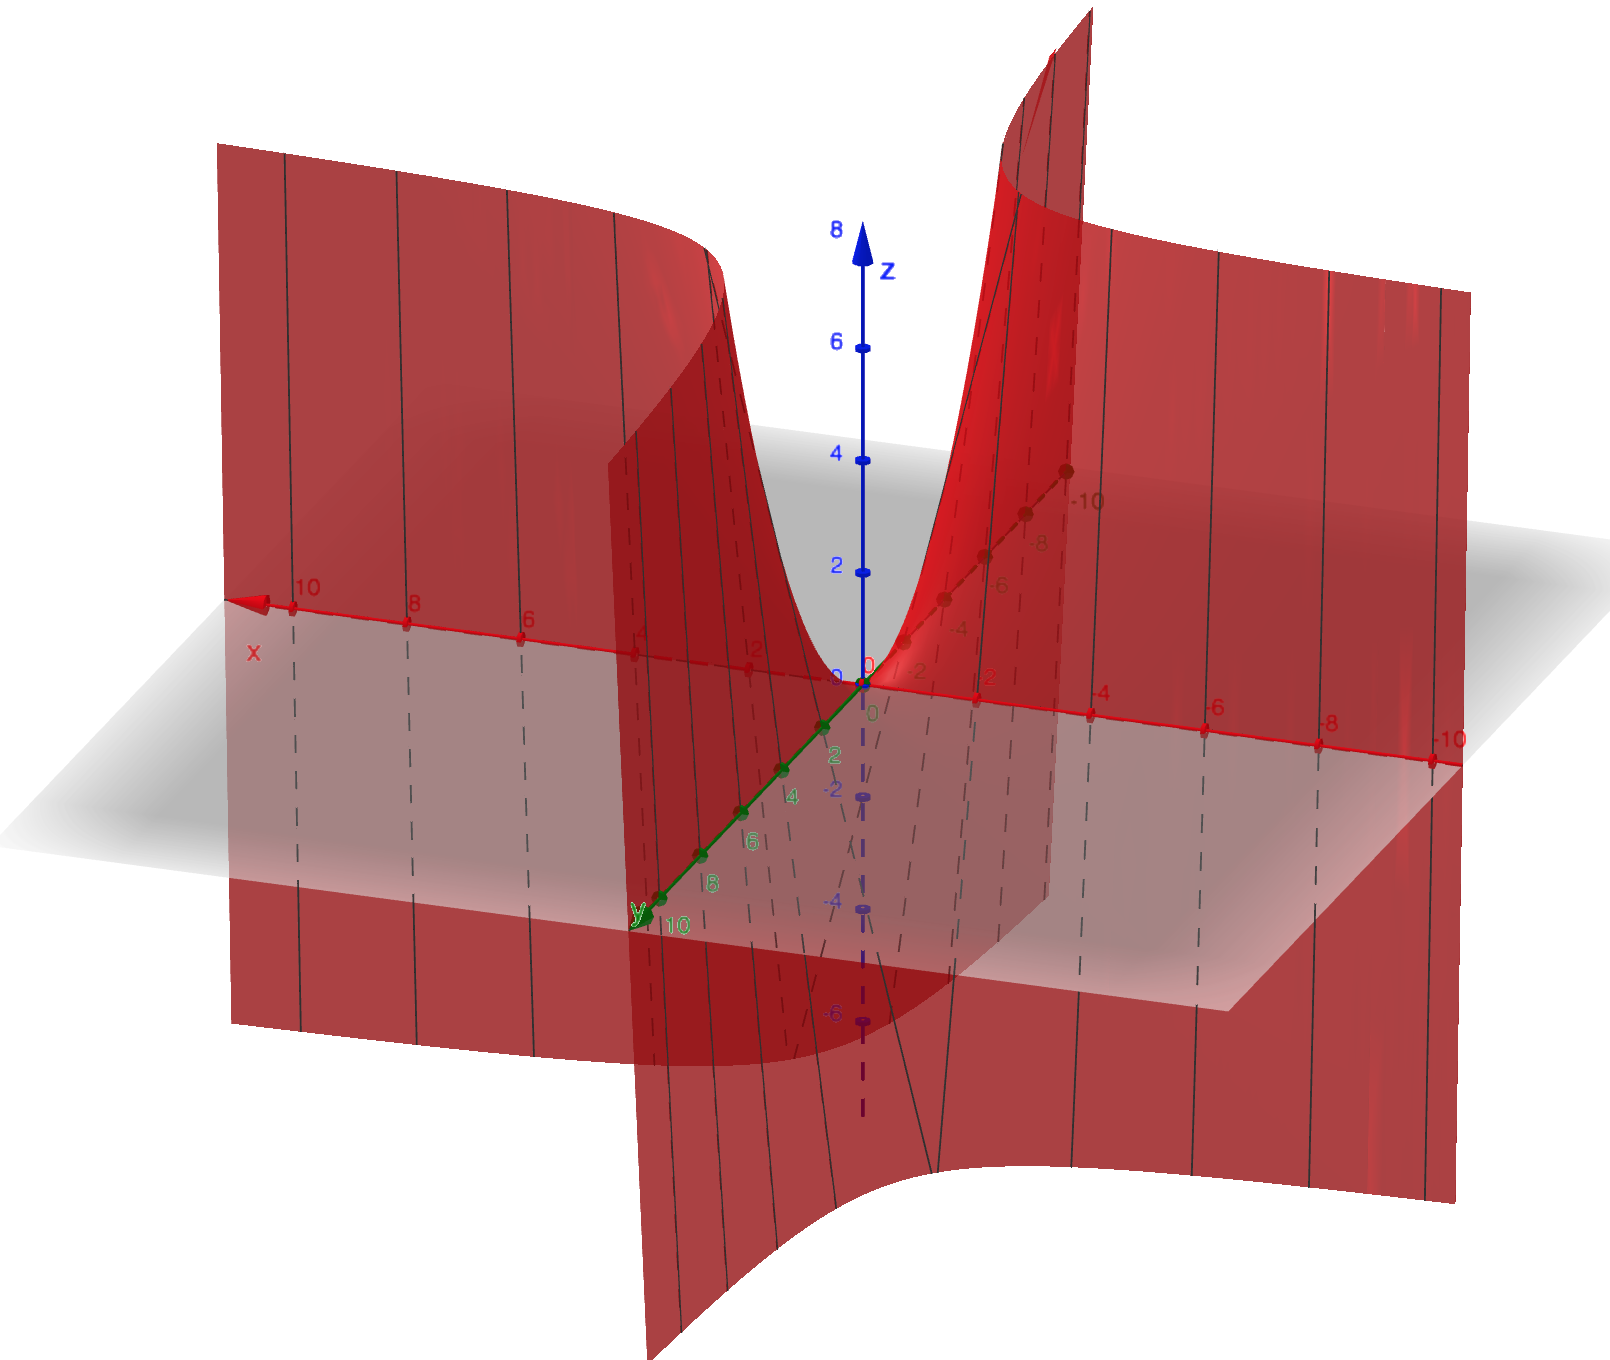
\includegraphics[width=0.4\textwidth]{2xy}
		}
		\subfigure[$g(x, y) = xsin(y)$, \quad $g(1, 1) = 0.017$]{%
			\label{fig:xsin(y)}
			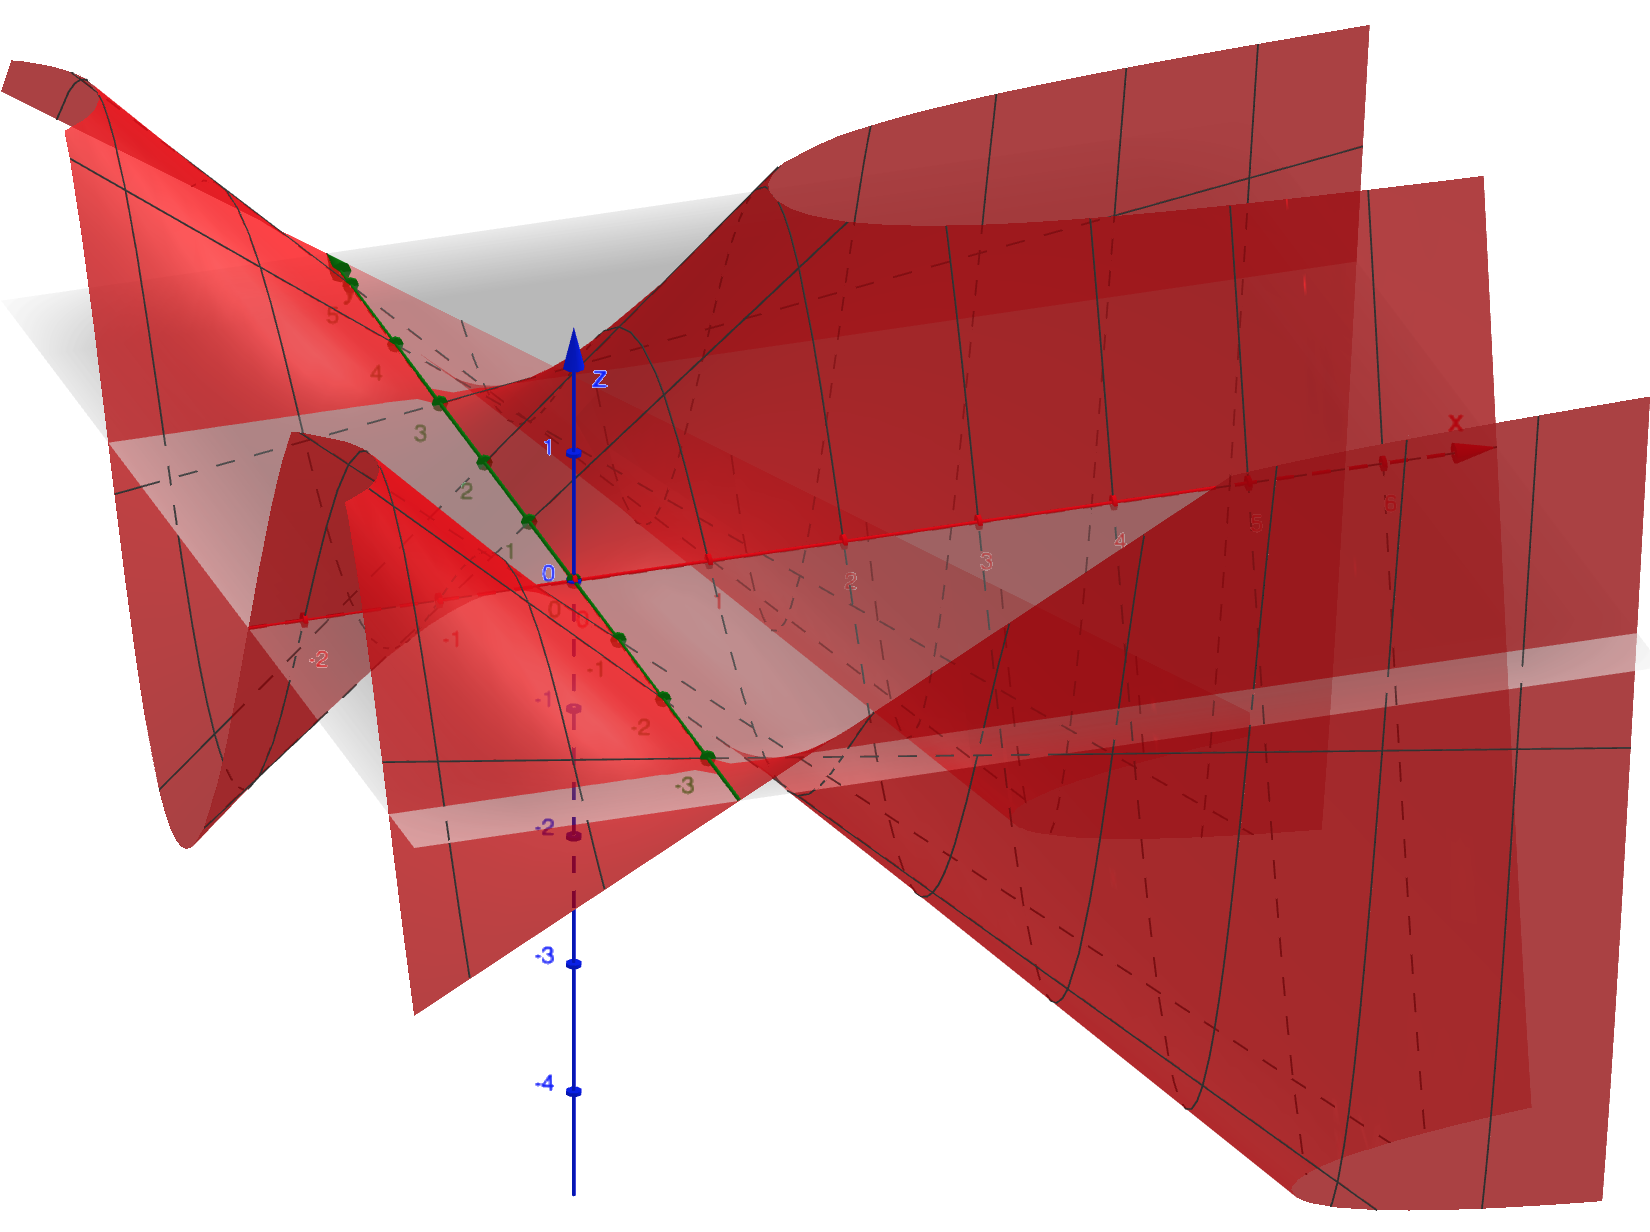
\includegraphics[width=0.4\textwidth]{xsin(y)}
		}
	\end{center}
	\caption{
		Different value functions for different functions.
	}
	\label{fig:ComparisonBetweenTwoFunctions}
\end{figure}

In addition to this, it became soon clear that the information concerning the number of remaining function' s soundings is redundant. It did not add any information to knowledge. In the implementation described above, the agent was in a terminal state when the number of remaining function soundings was equal to zero.

\paragraph{Second Step} The second step was globally equal to the first one except for two fundamental aspects. In the current step the possibility for the agent to make movements of different sizes was introduced. This possibility allowed its to reach the goal with a lower training time. 

The reward function was also redefined. It was equal to the percentage of proximity to the maximum of the function. It became soon clear that a so defined reward function was completely wrong. In a context of black-box optimization the maximum of the function is unknown and it was not possible to compute the percentage of proximity to the maximum.

\paragraph{Third Step} In the third step an additionally change to the previous one was made. At the end of each episode, the agent was artificially forced to restart from the coordinates of the previous episode's best rewarded epoch. Results given by the combination of the last two approaches resulted to be very fruitful in the context well-known function optimization but not in the context described in this thesis. This choice forced the agent to take a specific action, breaking, in so doing, for at least one time the concept of environment formalized through a Markov Decision Process.

\paragraph{Fourth Step} In the fourth step performances obtained through changes made in the second and third step were improved. This was possible imposing the agent to start each episode from the best rewarded epoch from all previous episodes.

\paragraph{Fifth Step} The fifth step is one of the most important because of innovations introduced. The first change made regarded actions. In this step the possibility for the agent to directly choose the size of the movement was introduced. There were still four different possible \textit{movement actions} :

\begin{itemize}
	\item Move North
	\item Move South
	\item Move West
	\item Move East
\end{itemize}

but the agent could select to move itself in one direction of :

\begin{itemize}
	\item \textit{movement amount};
	\item \textit{movement amount} $\times 2$;
	\item \textit{movement amount} $\times 3$.
\end{itemize}

The unit of measurement of \textit{movement amount} was the \textit{pixel}. The basic amount of movement was 40 pixels. The real movement amount over function was computed through algorithm \ref{algoPixel} in Chapter $3$. It was proved that using this set of \textit{action movements} the algorithm converged more quickly to the maximum of the function but the precision was lower. 

In addition to this, the possibility for the agent to distinguish between \textit{move action} and \textit{dig action} was removed. Each time the agent made a movement it also sounded the function obtaining a reward. The reward was positive if its proximity to the global maximum was in percentage $\ge 75\%$, negative in other cases. As already explained, the disadvantage of the last choice is that in the context described in this thesis the objective function is unknown so it is not possible to compute the percentage of proximity to the maximum.

\paragraph{Sixth Step} In this step the concept of \textit{delta} was introduced. \textit{delta} was computed as the difference between the value of the function sounded at time $t$ and the maximum value sounded until time $t$. 

In this step an higher control about \textit{exploration} and \textit{exploitation} was achieved. In order to do this a decreasing $\epsilon$ factor between episodes was introduced. Different decreasing functions were tested and it was clear that the best one was the logarithmic one. 

In this step the reward was still based on the concept of percentage with an engagement of the \textit{delta}. To be more specific if the \textit{delta} was $\le 0$ or the percentage was $\le 78\%$ the reward was negative, otherwise it was positive.

\paragraph{Seventh Step} In this step the definition of the reward function was improved. The concept of percentage of proximity to maximum was removed and a reward based exclusively on the difference between the sounded value function at time $t$ and the maximum until time $t$ was introduced. This was a little but fundamental adjustment because it removed a relevant mistake from the project.

\paragraph{Eighth Step} This step can be defined as an experimental step. Here the agent was made able to explore more. In order to do this the possibility to start each episode from a random point was introduced. Through this experiment it was proved that more exploration gave the possibility to prevent many limit cases but it did not always entail an improvement in algorithm performances in terms of time and precision.

\paragraph{Ninth Step} The current one is the second revolutionary step. It introduces two innovative elements: the \textit{parametric movement} and the \textit{stop action}.
As explained in chapter $3$, the parametric movement allows to compute the \textit{real agent's movement amount} keeping in consideration an approximation of function' s shape.

Speaking about the second innovation introduced,  it is important to say that when \textit{stop action} was selected, the simulation of the current episode was interrupted. Consequences from introduction of this new action were very interesting. Given a inadequate training space, the \textit{stop action} led to an immediate stop. This depended on the fact that rather than receiving more negative rewards before reaching a maximum better than the current one (i.e. the starting point itself), it computed that the optimal policy consisted in staying around the starting point itself, still moving according to a recurring pattern that minimizes the negative rewards.

\paragraph{Tenth Step} This represents the last step before the final version of the project. In this version the state was revolutionised. It was now composed of the last three angles of improvements computed as described in chapter $3$. Angles varied between $- \pi$ and $+ \pi$ because also a worsening is here considered. Angles were rounded to the nearest multiple of two. The choices introduced in this step were unexpectedly not fruitful. The failure depended on two factors. Last three angles as the unique component of the state were not enough and the rounding cannot be chosen a priori. The correct choice of rounding should depend on the \textit{Lipschitz Constant}. 

Let's consider a single-variable function $f(x)$ for $x$ inside a domain $D$. The magnitude of the slope of $f(x)$ for two points $(x_1, f(x_1))$ and $(x_2, f(x_2))$ is thus 

\begin{equation}
	|\dfrac{f(x_1)-f(x_2)}{x_1 - x_2}|.
\end{equation}

A non-negative real number $L$, which is the smallest upper bound of the slope is called the \textit{Lipschitz Constant} :

\begin{equation}
L = |\dfrac{f(x_1)-f(x_2)}{x_1 - x_2}| = sup|\dfrac{df}{dx}|.
\end{equation}

The Lipschitz Constant limits how fast the function can change. If there is no Lipschitz Constant, the function can change extremely fast without border, that is, the function becomes discontinuous\cite{Lipschitz}.

For multivariate function the \textit{Lipschitz Constant} is defined as:

\begin{equation}
L\textsubscript{x\textsubscript{n}} = sup|\dfrac{\partial f}{\partial x_n}|.
\end{equation}

\begin{figure} [h!]
	\centering
	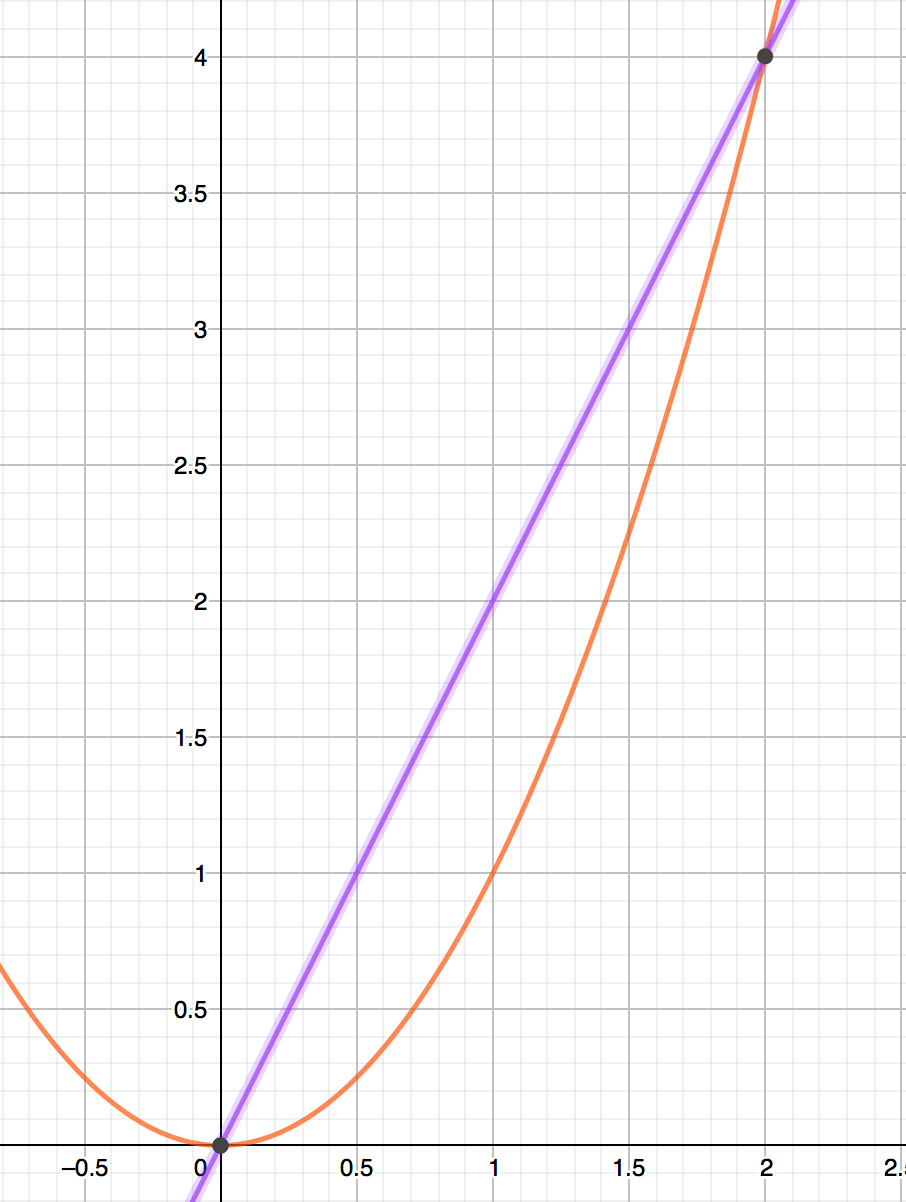
\includegraphics[width= 10cm, height = 10cm]{Lipschitz.png}
	\caption{Let's consider a $1d$-function $f(x) = x^2$ defined in the domain $x \in [0, 2]$. If $|\frac{df}{dx} f(x) | = 2x$, then $L = \sup |\frac{df}{dx}| = 2 \times 2 = 4$.}
	\label{fig:Lipschitz}
\end{figure}

